\documentclass[letterpaper, 11pt]{article} 

\usepackage{graphics,graphicx}
\usepackage{multicol} 
\usepackage{parskip}
\usepackage{amsmath}
\usepackage{multirow}
\usepackage[utf8]{inputenc}
\usepackage{fancyhdr}
\usepackage[title]{appendix}
\usepackage{wasysym}
\usepackage{url}
\usepackage{subcaption}

\usepackage[font=footnotesize,labelfont=small]{caption}
\captionsetup{width=0.85\linewidth}

\RequirePackage{geometry}
\geometry{margin=2cm}

\setlength{\parskip}{0.2cm}
\setlength{\parindent}{0pt}


\title{Project 1 Report: Bank-level Parallelism and Memory Controller Design}
\author{
Tai Duc Nguyen \\
ECEC 623: Advanced Topics in Computer Architecture
}
\date{\today}

\begin{document}

\maketitle


%----------------------------------------------------------------------------------------
%	ABSTRACT
%----------------------------------------------------------------------------------------


\rule{\textwidth}{1pt}

\begin{abstract}
	While Morse's Law has been true for modern processors, it does not apply to memory. Hence, in order for the memory speed to keep up with processing speed, many parallelism has to be exploited at many levels inside the memory of a von-Neumann computer. In this project, the effect of bank-level parallelism is explored along with 2 elementary memory controller design: FCFS - First Come First Serve, and FRFCFS - First Ready, First Come First Serve. 
\end{abstract}

\rule{\textwidth}{1pt}

\section{Experimental Setup}

In order to see how bank-level parallelism can improve memory speed, it is necessary to lay out a few constraints and metrics. The simulation assumes the following (but may not be limited to):
\begin{enumerate}
	\item DRAM Memory timings are:
	\begin{enumerate}
		\item Reading takes 53 clock cycles
		\item Writing takes 53 clock cycles
	\end{enumerate}
	\item PCM Memory timings are:
	\begin{enumerate}
		\item Reading takes 57 clock cycles
		\item Writing takes 162 clock cycles
	\end{enumerate}
	\item Maximum number of requests in the waiting queue is: 64
	\item The number of banks being tested are: 2, 4, 8, 16
	\item FR-FCFS loop searching for new request when the first one has bank-conflict can be done in 1 clock cycle
	\item A bank conflict of a memory request only counts once even though it could be queued and conflicted again in the next clock cycle
\end{enumerate}

From the assumptions above a simulation written in C is created. It first read a memory request from a memory trace, send such request to the "Waiting" queue. Once a request is in the queue, if the bank it targets is not busy, it will be pushed to the "Pending" queue and served in the next clock cycle. However, if the bank is busy, such request must wait until the bank is ready (in FCFS), or the program will find another request in the "Waiting" queue which targets a readied-bank.

The performance of bank-parallelism is then tested with FCFS \& FRFCFS controllers, and DRAM \& PCM Memory types. The metrics includes:
\begin{enumerate}
	\item Average Access Latency (\textbf{AAL})
	\item Number of Bank Conflicts (\textbf{BCF})
	\item Total Execution Time (\textbf{EXE})
\end{enumerate}

The 5 memory traces in this experiments are extracted from the following benchmarks: \textbf{503.bwaves\_r, 538.imagick\_r, 554.roms\_r, 557.xz\_r, and MP10}. The specifications for these benchmarks could be found in \url{https://www.spec.org/cpu2017/Docs/benchmarks/}

\section{Results and Discussion}

This section details the results from the simulation with graphs.

\begin{figure}[htb!]
	\centering
	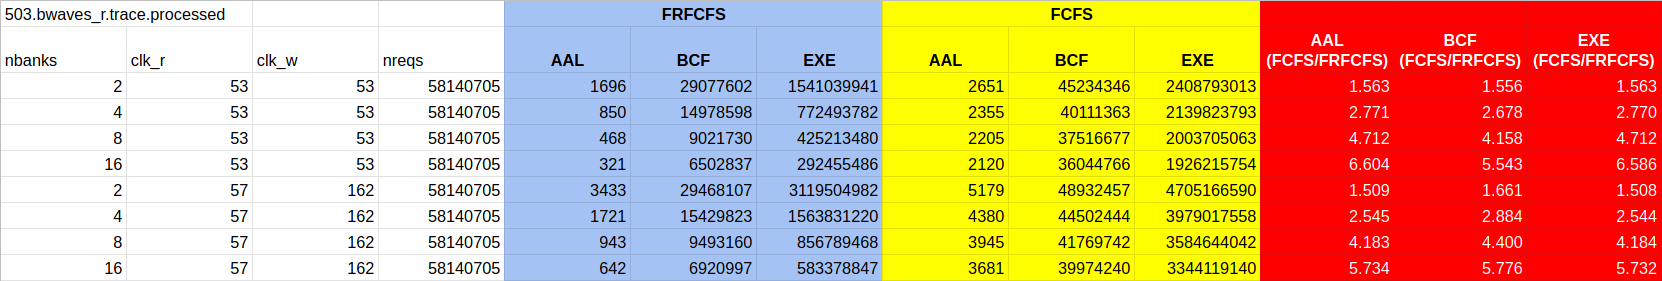
\includegraphics[width=1.0\linewidth]{503_results.png}
	\caption{Trace 503's simulation results, including improvement ratios between metrics of FCFS and FRFCFS}
	\label{fig1}
\end{figure}

\begin{figure}[htb!]
	\centering
	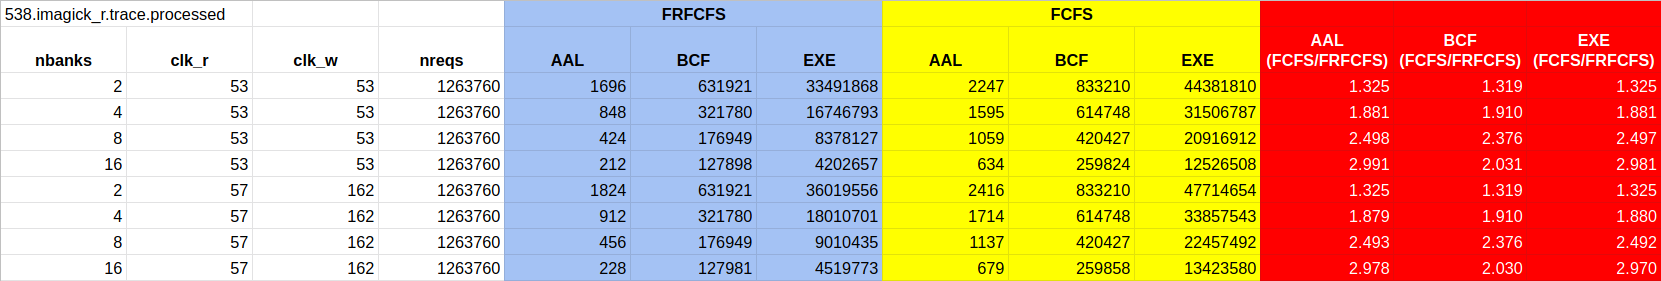
\includegraphics[width=1.0\linewidth]{538_results.png}
	\caption{Trace 538's simulation results, including improvement ratios between metrics of FCFS and FRFCFS}
	\label{fig2}
\end{figure}

\begin{figure}[htb!]
	\centering
	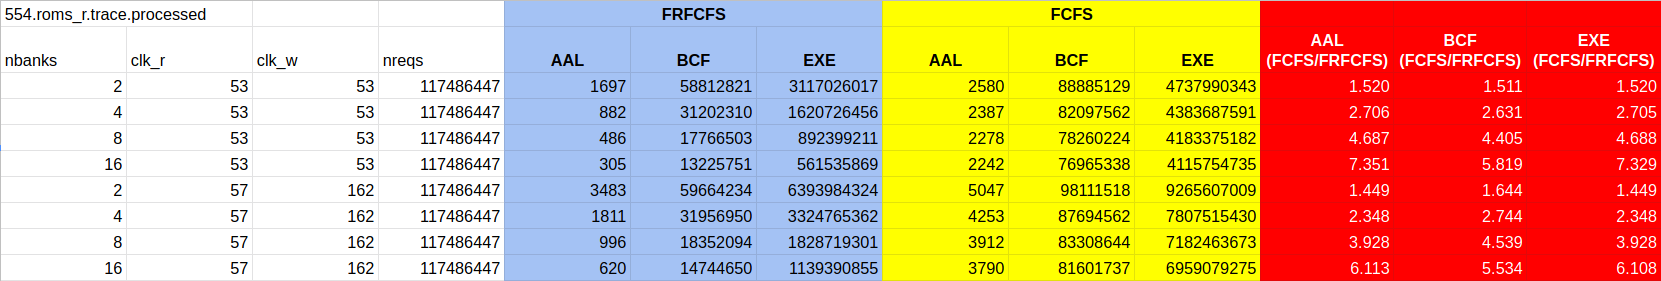
\includegraphics[width=1.0\linewidth]{554_results.png}
	\caption{Trace 554's simulation results, including improvement ratios between metrics of FCFS and FRFCFS}
	\label{fig3}
\end{figure}

\begin{figure}[htb!]
	\centering
	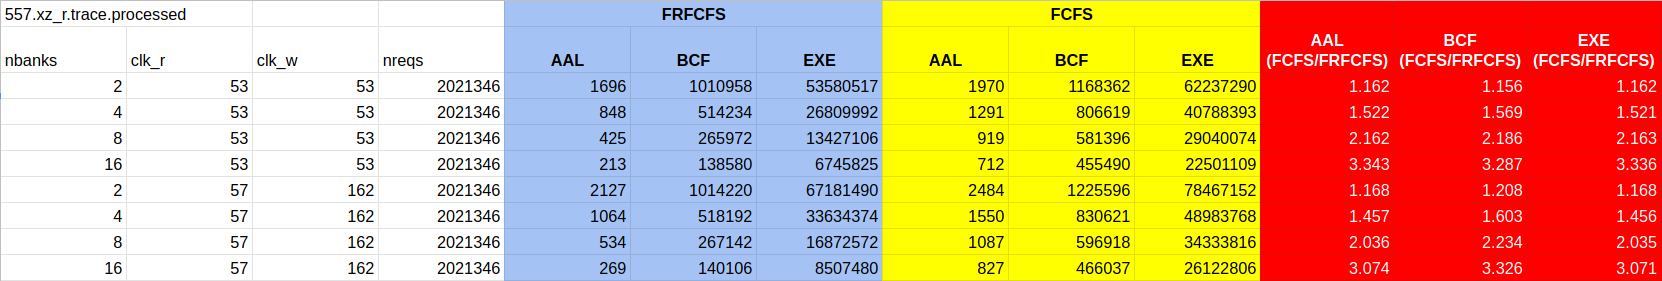
\includegraphics[width=1.0\linewidth]{557_results.png}
	\caption{Trace 557's simulation results, including improvement ratios between metrics of FCFS and FRFCFS}
	\label{fig4}
\end{figure}

\begin{figure}[htb!]
	\centering
	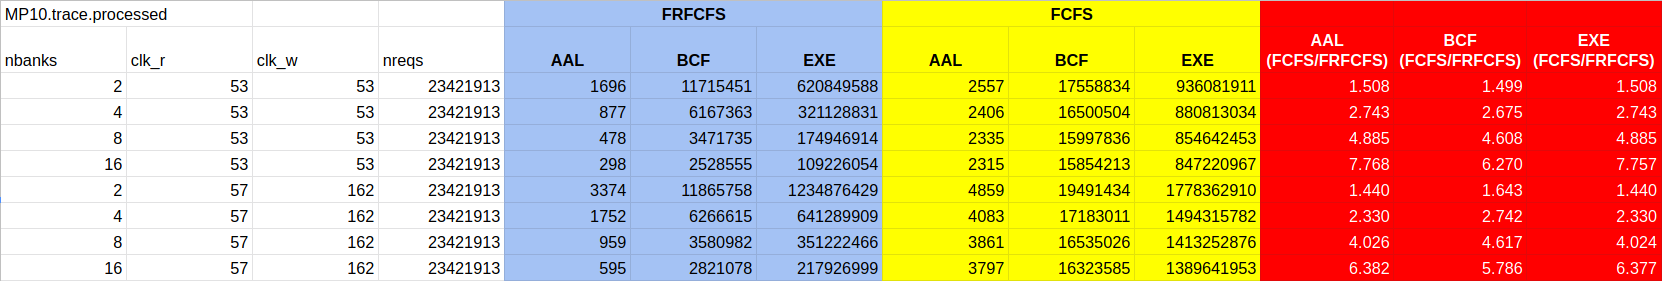
\includegraphics[width=1.0\linewidth]{MP10_results.png}
	\caption{Trace MP10's simulation results, including improvement ratios between metrics of FCFS and FRFCFS}
	\label{fig5}
\end{figure}

\begin{figure}[htbp!]
	\centering
	\begin{subfigure}[b]{.48\linewidth}
		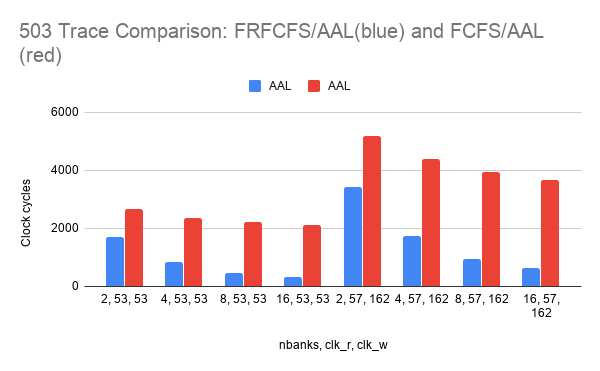
\includegraphics[width=\textwidth]{503_results_graph.png}
		\caption{Trace 503}
		\label{fig6a}
	\end{subfigure}
	\hfill %%
	\begin{subfigure}[b]{.48\linewidth}
		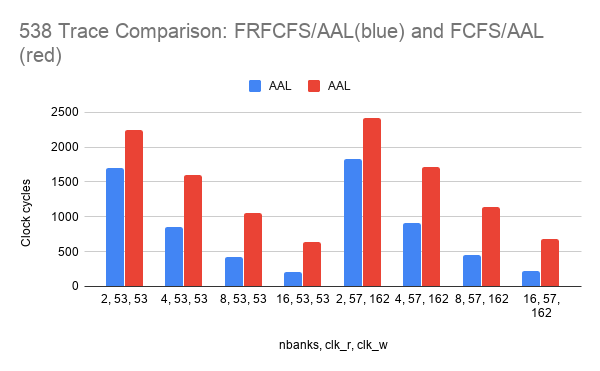
\includegraphics[width=\textwidth]{538_results_graph.png}
		\caption{Trace 538}
		\label{fig6b}
	\end{subfigure}
	\hfill %%
	\begin{subfigure}[b]{.48\linewidth}
		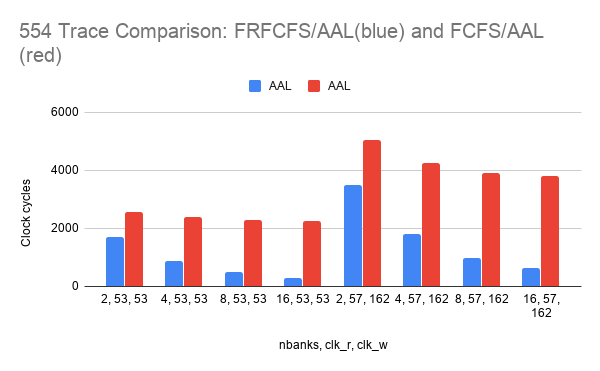
\includegraphics[width=\textwidth]{554_results_graph.png}
		\caption{Trace 554}
		\label{fig6c}
	\end{subfigure}
	\hfill %%
	\begin{subfigure}[b]{.48\linewidth}
		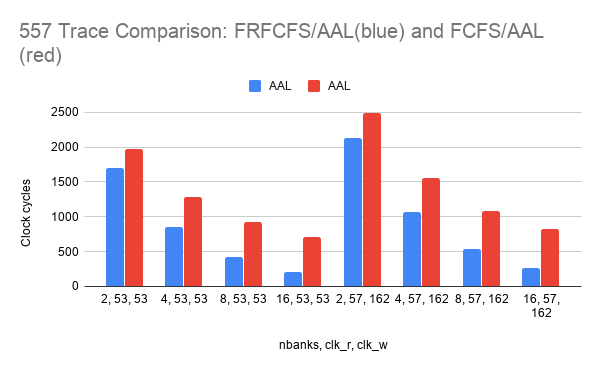
\includegraphics[width=\textwidth]{557_results_graph.png}
		\caption{Trace 557}
		\label{fig6d}
	\end{subfigure}

	\begin{subfigure}[b]{.48\linewidth}
		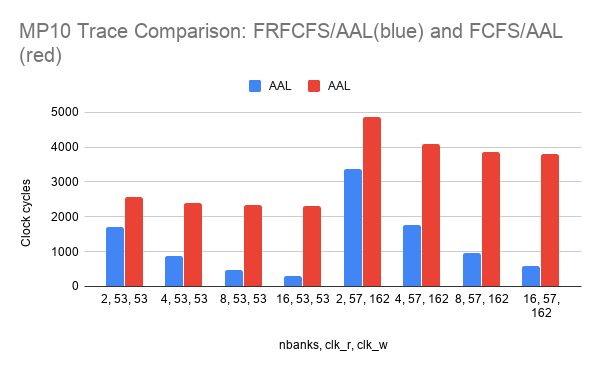
\includegraphics[width=\textwidth]{MP10_results_graph.png}
		\caption{Trace MP10}
		\label{fig6e}
	\end{subfigure}
\caption{Graph summary of simulations' results}
\end{figure}

\newpage
From these results, there are a few trends which emerge:
\begin{enumerate}
	\item AAL only slightly decreases with increasing number of banks for trace 503, 554 and MP10. This signifies that these programs are mostly trying to read or write to the same memory address (maybe in a loop). The memory accesses are not alocated equally across the banks.
	\item AAL decreases a long with increasing number of banks for trace 538 and 557. This tells that these 2 benchmarks includes memory accesses which are spread equally across the banks.
	\item PCM memory is much slower on average than DRAM memory.
	\item The higher the number of banks, the more significant of improvements seen in FRFCFS vs FCFS. In cases where there are 16 banks, the improvement is as large as 7.8 times. With a lower number of banks, the improvement is around 1.5 to 2 times. 
	\item FRFCFS provide such an improvement over FCFS because it keeps the Pending queue full most of the time, hence, saving many clock cycles by not stalling until the conflict is resolved.
	\item AAL, BCF and EXE are all directly proportional to one another.
\end{enumerate}

\textit{Graphical results are plotted on the next page.}
\end{document}